%%%
%%% Introduction
%%%
\section{Introduction} % in progress
\label{introduction}
\subsection{Motivation}
\begin{itemize}
    \item so many people suffer from back problems...: 
    \begin{itemize}
        \item 60\% - 90\% of people will suffer from low back disorders at some point in their life \cite{osha2000facts}
        \item 30\% of European workers suffer from back pain \cite{osha2000facts}
        \item back pain tops the list of all reported work-related disorders \cite{osha2000facts}
    \end{itemize}
    \item so many people work on laptops/computer on a daily basis: 57 \% of all employees in EU use computers at their workplace (2019) \cite{eurostat_comp_use}
    \item "Exposure to ergonomic risks factors represents one of the major occupational safety and health problems in the EU today. Repeated exposure to these risks can result in work-related musculoskeletal disorders — one of the most serious and widespread work-related illnesses, which give rise to major cost burden for individuals, businesses and society in general." \cite{osha2019msd}
\end{itemize}
%%% Problemanalyse

%\begin{figure}[htpb]
%\centering
%  \subcaptionbox{Baseline of PR\label{fig:us2baseline}}{
%   \includegraphics[width=0.225\textwidth]{media/IMG_0063minimized.png}
%  }
%  \subcaptionbox{Full reduction level of PR\label{fig:us2fullreduction}}{
%   \includegraphics[width=0.225\textwidth]{media/IMG_0064minimized.png}
%  }
%  \caption{Reduction levels}
%  \label{fig:us2reductionlevels}
%\end{figure}


%%%
%%% Related Work
%%%
\section{Related Work} % in progress
\label{related-work}
% Ähnliche Produkte

% Gleiches Konzept, aber ausschließlich regelbasiert

"Posture monitoring and improvement for laptop use."~\cite{demmans2007posture}

“Sit straight (and tell me what I did today): a human posture alarm and activity summarization system”~\cite{jaimes2005sit}

\section{Technology} % in progress
\subsection{Components} % in progress
\begin{itemize}
    \item PoseNet model
    \item rule-based system
    \item feedback system
    \item statistics
\end{itemize}

\section{Medical consultation} % in progress

%%%
%%% User Study 1
%%%
\section{User Study: Examining the effects of ...} % in progress
\label{user-study-1}
- examining the effects of improving posture habits with body pose.
- examining the usability of body pose app

\subsection{Study Design} % in progress
\label{us1-study-design}
- laboratory study
- controlled variables: working on our own tested devices, everyone has same working environment (due to executing it at Hyve)


- Evaluating web-based user interfaces is not trivial. % but has been carried out before.
Researchers have used different metrics to identify various relevant aspects in the past. These can be (among others) the workload that a system provokes~\cite{hart1988development,hart2006nasa}, the creativity support that it provides~\cite{cherry2014quantifying}, the sense of control a user perceives~\cite{dong2015development}.

\subsection{Study Tasks} % in progress
\label{us1-tasks}
We defined three phases within the user study. Phase one should give the participants an overview of the features BodyPose and should encourage to explore them on their own. As BodyPose is designed for background usage, phase two simulates an every day's work task. Lastly, the participants are invited to fill in a survey consisting of two questionnaires in order to ask for feedback regarding personal information as well as user experience and subjective perception of the study task itself.
\begin{description}

\item[Task A]
    - activate camera feed
    - deactivate and reactivate browser notifications
    - try different settings within body pose

\item[Task B] (simulation of working task / light-moderate workload):
    - while using body pose in background: write a text (recipe) and add a picture (internet research)

\item[Surveys]
    survey 1 (Google survey)
        - personal questions (age, weight, back pain history, ...)
        - questions regarding task 1: 

\end{description}

\subsection{Measurements} % in progress
\label{us1-measurements}

We utilised an extended version of the NASA-TLX~\cite{hart2006nasa} to collect quantified data at end of the task. The questionnaire measured workload, sense of control and creativity support. The Task-Load Index (TLX) from NASA~\cite{hart2006nasa} measured the subjective amount of workload experienced by the participants. The sense of control scale by Dong et al.~\cite{dong2015development} adapted to a 20-point rating scale measured perceived control. Lastly, Creativity Support Index by Cherry et al.~\cite{cherry2014quantifying}, limited to exploration, motivation and enjoyment dimensions measured the creativity support.

\subsection{Procedure} % in progress
\label{us1-procedure}
\subsection{Preparation} % in progress
- we prepared three of our laptops: Browser with 3 tabs: Webapp, survey1, survey2 

\subsection{Conduct} % in progress
- after welcoming the participants, each of them got a sheet of paper with the in \ref{us1-tasks} described instructions written on it. -were seated in front of one of our laptops, -were indicated on which tabs to find webapp, survey1, survey2 -then indicated to pls follow the instructions and after completing all to fill in both surveys. No time constrain was added.  

\subsection{Participants} % in progress
\label{us1-participants}
- 3 participants, 2 male 1 female, students in the field of computer science, average age 24 from 23 - 27,


\subsection{Data Analysis and Results} % in progress
\label{us1-data-analysis-results}
<As shown in \ref{fig:us-gs-shortterm}, bodypose motivates probands to adjust their posture if app detects misalignment.> 

\begin{figure}[hbp]
\centering
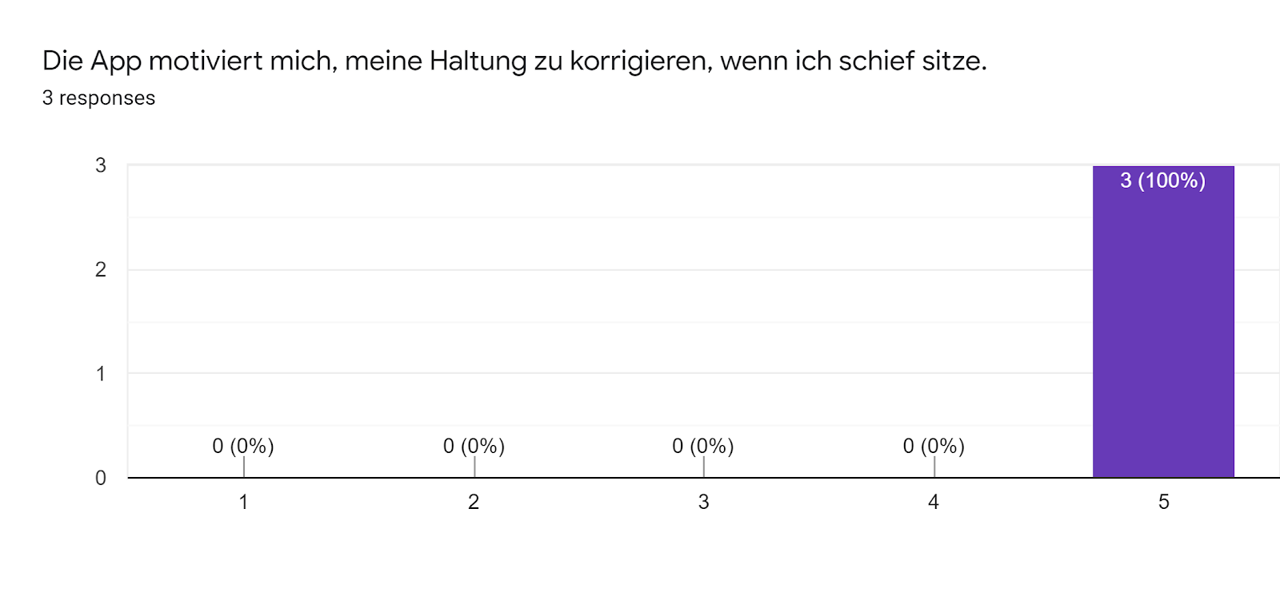
\includegraphics[width=\linewidth]{media/us-gs-shortterm-motivation-results.png}    
\caption{Results Shortterm Motivation, N=3}
\label{fig:us-gs-shortterm}
\end{figure}

<As shown in \ref{fig:us-gs-longterm}, bodypose seems to increase motivation in participants to take care of their posture in longterm.>

\begin{figure}[hbp]
\centering
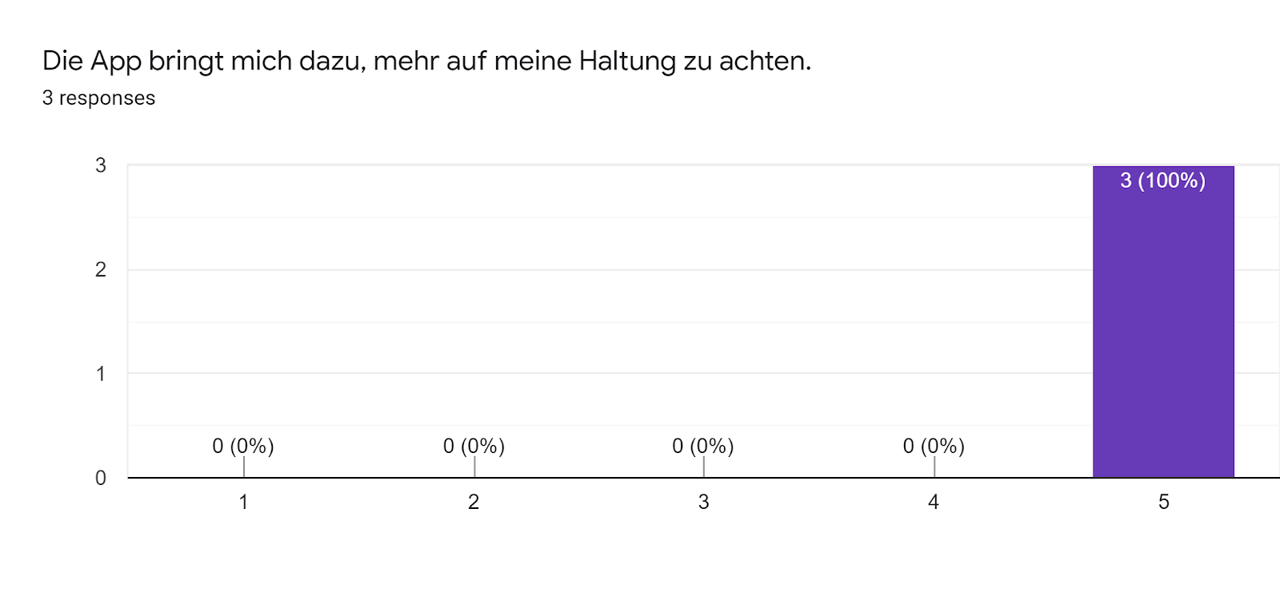
\includegraphics[width=\linewidth]{media/us-gs-longterm-motivation-results.png}    
\caption{Results Longterm Motivation, N=3}
\label{fig:us-gs-longterm}
\end{figure}


- graph: results extended NASA-tlx study
<As shown in \ref{fig:ext-nasa-results}, probands felt [...] while executing user study task>

\begin{figure}[hbp]
\centering
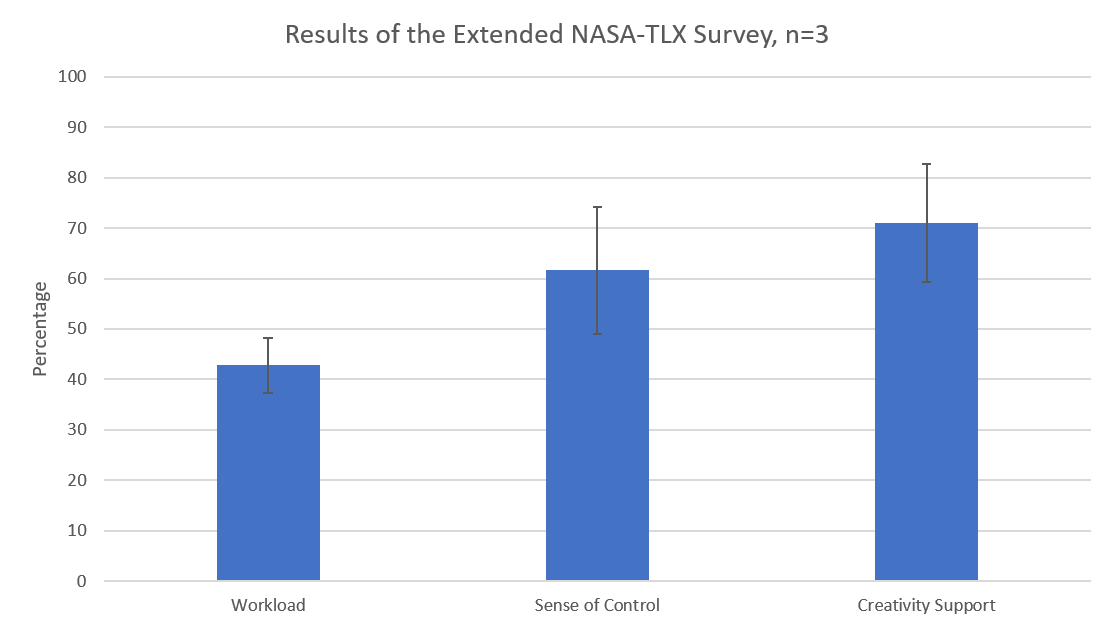
\includegraphics[width=\linewidth]{media/us-ext-nasa-tlx-results.png}    
\caption{Results Extended NASA TLX Survey, N=3}
    \label{fig:ext-nasa-results}
\end{figure}

%%%
%%% Discussion and future work
%%%
\section{Discussion} % in progress
\label{discussion-future-work}


\subsection{User Study Procedure}
As only three participants took part in our user study, the results shown in \ref{us1-data-analysis-results} are statistically not representative. Furthermore, execution of the user study did not strictly follow the study protocol described in \ref{us1-procedure}: Since our participants were aware they were being observed not only by us, but also by our mentors and colleagues, their behaviour might also not have been representative. Additionally, participants were not isolated from each other, so they did not perform their tasks independently. Lastly, since we recruited the participants from amongst our co-students, it can not be ruled out that personal bias(es) might have had an influence on the result.
% It should be noted, however, that this study is considered to be a test run. To gain reliable results and insights, a higher number of participants, as well as a more controlled and isolated setup are required.

%%%
%%% Conclusion
%%%
\section{Conclusion} % in progress
\label{conclusion}

% \lipsum[2-4]
\section{Future Work}
\begin{itemize}
    \item let model learn rule-based system
\end{itemize}
There are several potential future avenues worth pursuing in order to enhance and improve the functionality of BodyPose: To allow for a more personalised user experience, users should be able to create an account and save not only their settings (such as threshold values), but also calibration and session data (such as statistics). Furthermore, implementing a user identification system via face detection might prove helpful for robustness: since BodyPose uses PoseNet's single-pose detection algorithm, the system can not handle situations robustly where multiple persons are visible to the camera. Identifying users with face detection could mitigate this problem, as the system could be modified to only evaluate the pose of persons who can be identified as the currently logged in user. Another avenue for improving robustness, as well as accuracy, lies in replacing the pose detection model itself: PoseNet detects poses in two dimensions, but there are also models that can detect poses in three dimensions, even from two-dimensional input, such as in \cite{Arnab_2019}. This model shows improved robustness and accuracy when compared to two-dimensional pose detection. However, due to the added complexity, this could potentially result in a trade-off regarding performance.

\appendix
%Appendix A
%\section{User Study 1: Visual search task}

%\begin{figure}[hbp]
%\centering
%\includegraphics[width=\linewidth]{media/us1.png}    
%\caption{Layer setup}
%\label{fig:us1layers}
%\end{figure}

\begin{acks} % in progress
  The authors would like to thank all three participants for their participation in the user study, as well as Dr. Marco Meier, HYVE and TAWNY staff for their mentoring.
\end{acks}